\section{Bus Buffering and Latching}
\begin{itemize}
  \item The address / data bus on the $\mu P$ is multiplexed (shared) to reduce the number of pins, which on the other hand, burdens with the task of extracting or \textit{demultiplexing} info from these pins
  \item \textbf{Why not leave the buses multiplexed?}
  \begin{itemize}
    \item Memory and I/O require that the address remains valid and stable throughout a read or write cycle. If the busses are multiplexed, the address can get changed causing read or write in wrong locations.
  \end{itemize}

  \item All computer systems have three types of buses:
  \begin{enumerate}
    \item \textbf{Address bus}: Provides memory address or I/O port numbers
    \item \textbf{Data bus}: Transfers data between $\mu P$ and the memory I/O
    \item \textbf{Control bus}: Provides control signals to memory and I/O
  \end{enumerate}
\end{itemize}
% \newpage
\section{Basic of Demultiplexing}
\begin{figure}[h!]


  \tikzset{every picture/.style={line width=0.75pt}} %set default line width to 0.75pt

  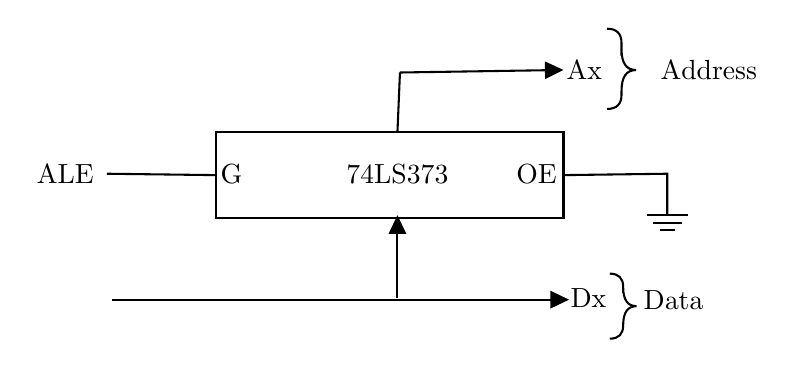
\begin{tikzpicture}[x=0.75pt,y=0.75pt,yscale=-1,xscale=1]
  %uncomment if require: \path (0,300); %set diagram left start at 0, and has height of 300

  \draw    (242.67, 120) rectangle (410, 161.33)   ;
  \draw    (331.22,91.23) -- (330,120) ;


  \draw    (331.22,91.23) -- (408,90.03) ;
  \draw [shift={(410,90)}, rotate = 539.1] [fill={rgb, 255:red, 0; green, 0; blue, 0 }  ][line width=0.75]  [draw opacity=0] (8.93,-4.29) -- (0,0) -- (8.93,4.29) -- cycle    ;

  \draw   (430.97,108.8) .. controls (435.64,108.8) and (437.97,106.47) .. (437.97,101.8) -- (437.97,100.04) .. controls (437.97,93.37) and (440.3,90.04) .. (444.97,90.04) .. controls (440.3,90.04) and (437.97,86.71) .. (437.97,80.04)(437.97,83.04) -- (437.97,77.13) .. controls (437.97,72.46) and (435.64,70.13) .. (430.97,70.13) ;
  \draw    (410,140.67) -- (460,140) -- (460,160) ;


  \draw    (190,140) -- (242.67,140.67) ;


  \draw    (192.67,200.67) -- (410.67,200.67) ;
  \draw [shift={(412.67,200.67)}, rotate = 180] [fill={rgb, 255:red, 0; green, 0; blue, 0 }  ][line width=0.75]  [draw opacity=0] (8.93,-4.29) -- (0,0) -- (8.93,4.29) -- cycle    ;

  \draw   (432.3,219.47) .. controls (436.6,219.47) and (438.75,217.32) .. (438.75,213.02) -- (438.75,213.02) .. controls (438.75,206.87) and (440.9,203.8) .. (445.2,203.8) .. controls (440.9,203.8) and (438.75,200.73) .. (438.75,194.58)(438.75,197.35) -- (438.75,194.58) .. controls (438.75,190.28) and (436.6,188.13) .. (432.3,188.13) ;
  \draw    (330,200) -- (330,162) ;
  \draw [shift={(330,160)}, rotate = 450] [fill={rgb, 255:red, 0; green, 0; blue, 0 }  ][line width=0.75]  [draw opacity=0] (8.93,-4.29) -- (0,0) -- (8.93,4.29) -- cycle    ;

  \draw    (470,160) -- (450,160) ;


  \draw [line width=0.75]    (467.11,163.62) -- (453.11,163.62) ;


  \draw [line width=0.75]    (463.61,167.12) -- (456.61,167.12) ;



  \draw (330,140) node  [align=left] {74LS373};
  \draw (250,140) node  [align=left] {G};
  \draw (397,140) node  [align=left] {OE};
  \draw (420,90) node  [align=left] {Ax};
  \draw (480,90) node  [align=left] {Address};
  \draw (170,140) node  [align=left] {ALE};
  \draw (422,200) node  [align=left] {Dx};
  \draw (463,201) node  [align=left] {Data};


  \end{tikzpicture}

  \caption{Using the 74LS373}
\end{figure}
\newpage
\subsection{Demultiplexing 8088}
\begin{figure}[h!]
  \includegraphics[width = 0.8\textwidth]{./figures/8088_demux.png}
  \caption{The 8088 microprocessor shown with a demultiplexed address bus. This is the
model used to build many 8088-based systems.}
  \label{}
\end{figure}
\begin{itemize}
  \item \textbf{74LS373} latches (OE for output enable and G or LE for latch enable inside) are used to demultiplex address/data bus connections and the address/status bus connections.
  \item \textbf{74LS373} passes inputs to outputs like wires when \textbf{ALE} is logic 1; when \textbf{ALE} is logic 0, the latches remember the inputs at the time of the change to logic 0.
\end{itemize}

\subsection{Demultiplexing 8086}
\begin{figure}[h!]
  \includegraphics[width = 0.8\textwidth]{./figures/8086_demux.png}
  \caption{The 8086 microprocessor shown with a demultiplexed address bus. This is the
model used to build many 8086-based systems.}
  \label{}
\end{figure}
\begin{itemize}
  \item Difference from 8088 AD15 - AD8 and $\overline{BHE}/S7$ is that $\overline{BHE}$ selects a high-order memory bank in a 16-bit memory system in 8086.
\end{itemize}
\newpage
\section{Buffered System }
\begin{itemize}
  \item If more than 10 unit loads are attached to any bus pin, the entire $\mu P$ system must be buffered (Buffer provides amplification in a digital circuit to drive output loads enabling more TTL unit loads to be driven)
  \item The \textit{demultiplexed} pins are already buffered by the \textbf{74LS373} latches.
  \item A fully buffered signal will introduce a timing delay, which causes no difficulty unless memory or I/O devices are used that function at near the maximum speed of the bus.
\end{itemize}

\subsection{Fully Buffered 8088}
\begin{figure}[h!]
  \includegraphics[width = 0.8\textwidth]{./figures/8088_fully_buff.png}
  \caption{A fully buffered 8088 microprocessor.}
  \label{}
\end{figure}
\begin{itemize}
  \item \textbf{74LS244}: Octal buffer
  \item \textbf{74LS245}: Octal bidirectional buffer

\end{itemize}


\subsection{Fully Buffered 8086}
\begin{figure}[h!]
  \includegraphics[width = 0.8\textwidth]{./figures/8086_fully_buff.png}
  \caption{A fully buffered 8086 microprocessor.}
  \label{}
\end{figure}
\newpage
\subsection{Number of chips required for fully buffered microprocessor}
\begin{table}[h!]
\centering
\begin{tabular}{ |p{1cm}|p{3cm}||p{4cm}||p{1cm}| }
\hline
$\mu P$ & \textbf{74LS244} (Octal buffer) & \textbf{74LS245} (Octal bidirectional buffer) & \textbf{74LS373} \\
\hline
8088 & 2  & 1 & 2\\
8086 & 1  & 2 & 3\\
\hline
\end{tabular}

\caption{Number of chips required for fully buffered microprocessor}
\label{table:4}
\end{table}
